\documentclass[12pt]{article}

\newcommand{\E}[1]{{\mathbf{E}[#1]}}
\newcommand{\Prob}[1]{{\mathbf{Pr}[#1]}}
\newcommand{\ProbSub}[2]{{\mathbf{Pr}_{#1}[#2]}}
\newcommand{\Var}[1]{{\mathbf{Var}[#1]}}
\newcommand{\Cov}[1]{{\mathbf{Cov}[#1]}}

\usepackage[authoryear,round]{natbib}
\usepackage{amsmath}
\usepackage{graphicx}
\usepackage{comment}
\usepackage{url}

\usepackage{subfigure}

\begin{document}

\date{}
\title{Relaxing The Closed World Assumption in Distant Supervision with a Generative Model of Corpora and Databases}
\author{}
\maketitle

\bibliographystyle{plainnat}

\section{Challenges}
\begin{description}
  \item[{\bf Incomplete Databases}]:
    \begin{itemize}
    \item Facts are often omitted from databases.
    \item This can result in misleading training data, for example supposing \emph{Amazon} is listed as a {\sl COMPANY},
      but not a {\sl LOCATION}, the sentence \emph{I am flying to the Amazon} would be mis-labeled as referring
      to a {\sl COMPANY}.
    \end{itemize}
  \item[{\bf Missing Entries} (\emph{Semi-Supervised Distant Supervision})]:
    \begin{itemize}
      \item Many items (e.g. entities, or entity-pairs) will not appear at all in the database
      \item If we are sufficiently confident, extractions involving these entities should be treated as if they were added to the database
        and used for further Distant Supervision.
        %TODO: Example
    \end{itemize}
\end{description}

\section{Solution}
To address both of these challenges, I believe we should investigate an approach based a generative model of both the text and the database which
preserves ambiguity over which facts are true/false rather than assuming all facts in the database are true, and all facts not in the database
are false (closed world assumption).

\subsection{Background: Previous Approach}
In previous work \citep{Ritter11}, we proposed an approach to distant supervision based on a Bayesian Network (Latent Dirichlet Allocation) representation of our data
in connection with a set of constraints on it's parameters.  More specifically:
\begin{itemize}
  \item We investigated weakly supervised named entity classification (e.g. input=extracted named entities and contexts + database, output=model and classification of named entities)
  \item Entities are modeled as mixtures of types (analogy from topic modeling: entities $\rightarrow$ documents, contexts $\rightarrow$ words, types $\rightarrow$ topics.)
  \item The set of possible types for each entity are constrained based on it's possible types according to a set of mutually exclusive dictionaries gathered from Freebase.
\end{itemize}

\begin{figure}
  \centering
  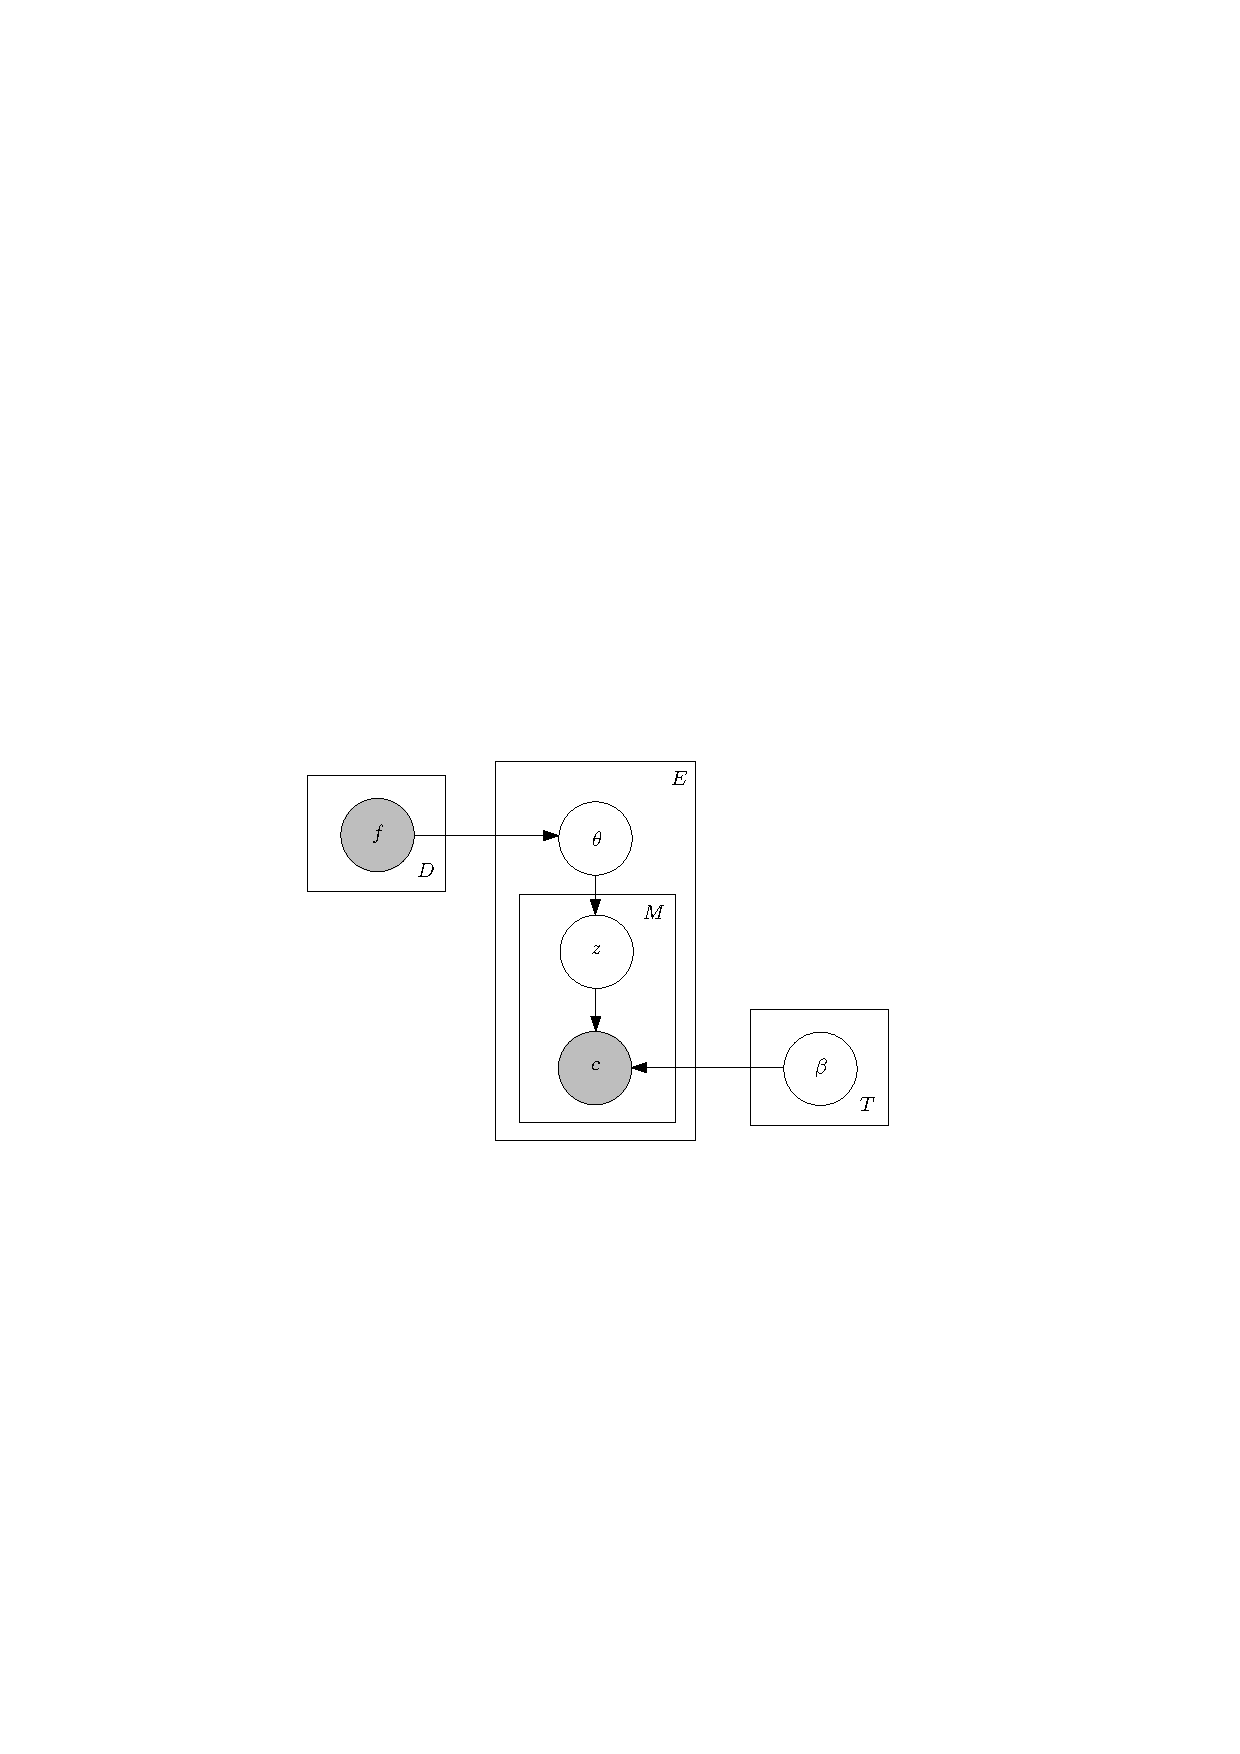
\includegraphics{llda.pdf}
  \caption{{\bf Distant Supervision With Topic Models}.  Mentions $M$ of entity $E$ are modeled as a mixture over types $\theta_E$.  The set of possible types
  for each entity is constrained by facts $f$ which relate to that entity.  Contexts $c$ are drawn from the multinomial, $\beta_{z_i}$ associated with type $z_i=T$.}
  \label{llda}
\end{figure}

Figure \ref{llda} presents a graphical model representation of this story for the data.


\subsection{Proposed Approach}
To avoid assuming facts not contained in the database are false, consider the following approach:

\begin{itemize}
  \item Introduce a hidden variable $g$ for each possible fact (including those not found in the database)
  \item Constrain the parameters $\theta$ based on the $g$'s instead of directly on the observed facts in the database.
  \item Model the probability of facts observed in the database conditioned on $g$.
\end{itemize}

The first part (constraining $\theta$ based on $g$) is the same as before.  The distribution $P(f|g)$ could be modeled as follows:
\begin{itemize}
  \item If $g$ is false, then $P(f|g) = 0$
  \item Otherwise $P(f|g) = \gamma$ where $\gamma$ could be a dictionary dependent parameter (e.g. it makes sense that some dictionaries have better coverage than others).
    For example, we are unlikely to extract any new Egyptian Pharaohs, but we are likely to identify new Movies, Athletes, etc...
\end{itemize}

\begin{figure}
  \centering
  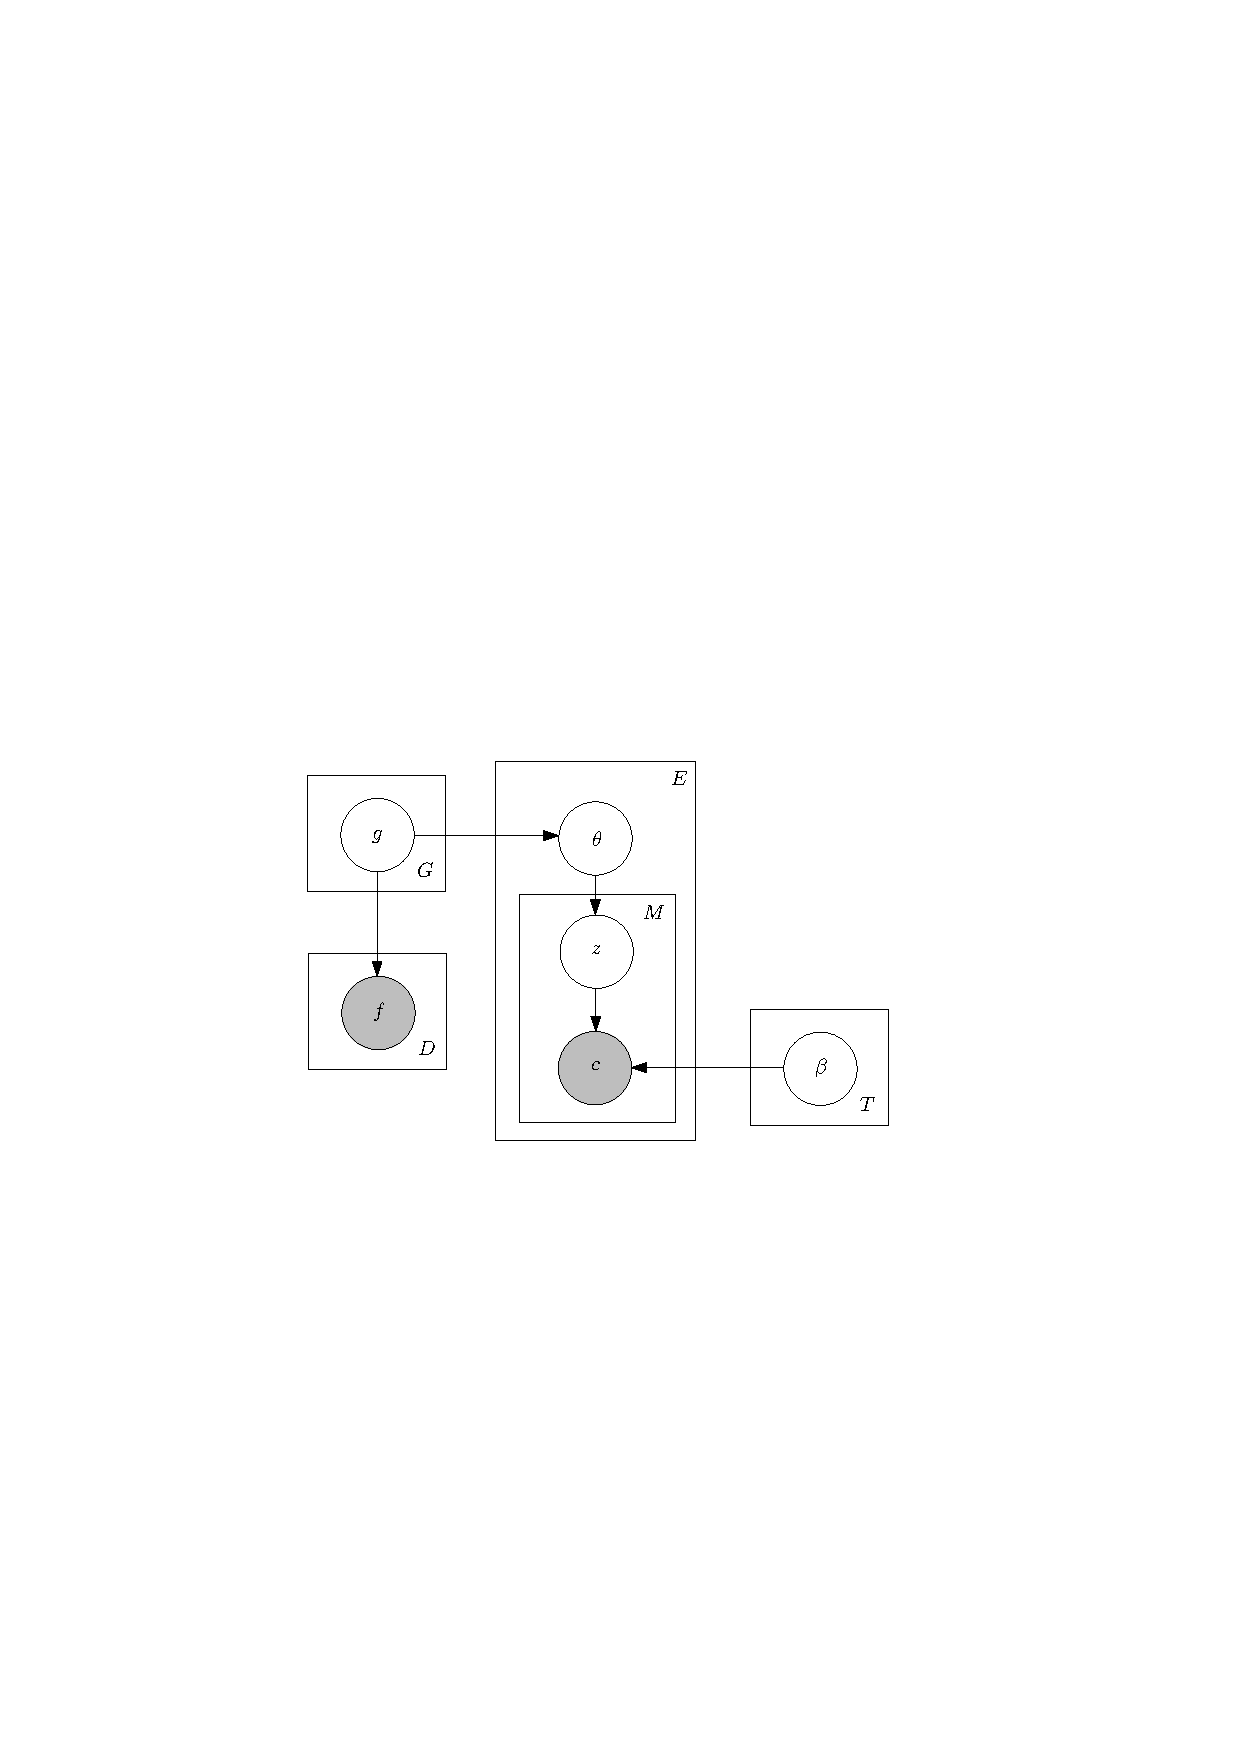
\includegraphics{glda.pdf}
  \caption{{\bf Distant Supervision Without the Closed World Assumption}.  Now parameters $\theta$ are constrained by hidden variables $g$.  Observed facts in the database
    are also conditioned on $g$.  See Figure \ref{llda} for additional details.}
\end{figure}

\subsection{Inference}
Inference will become slightly more complicated in this model, because when the $g$ variables are re-sampled, some of the $z_i$'s may need to be changed
in order to preserve the constraints.  I believe the sampling should be relatively straightforward to accomplish in this fashion using an appropriate proposal distribution.

\bibliography{bib}
\end{document}
